% !TEX root = ../lectures.tex
\section{The Grammage Pillar}
\label{sec:pillar}

\begin{figure}[t]
\centering
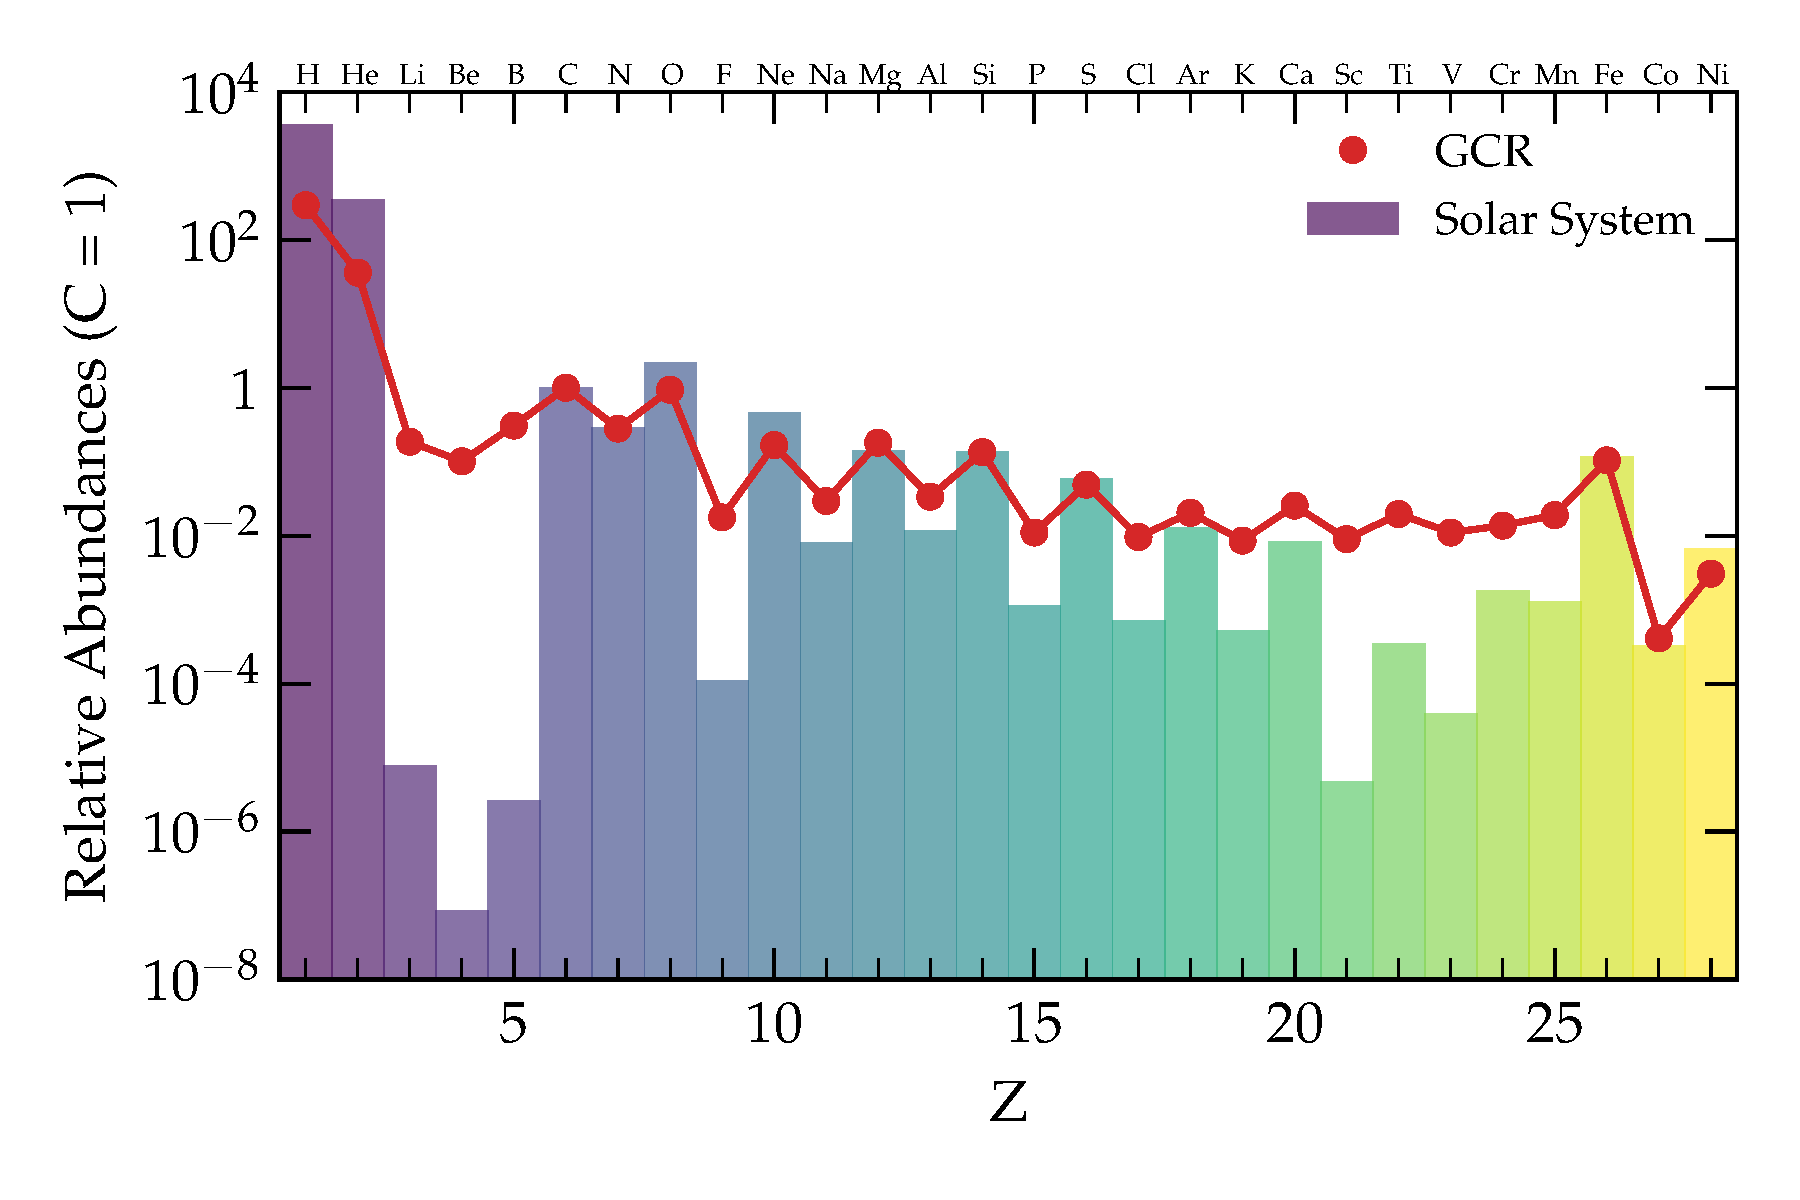
\includegraphics[width=0.6\textwidth]{figures/composition.pdf} 
\caption{Relative abundances of elements as a function of atomic number (Z) for Galactic Cosmic Rays (GCR)~\cite{} and the Solar System~\cite{}. The data highlight significant differences in the elemental composition between cosmic ray sources and the solar system medium, with abundances normalized to carbon (C=1).}
\label{fig:composition}
\end{figure}

The nuclear composition of cosmic rays (CRs) provides compelling evidence that GeV-TeV cosmic rays do not travel in straight lines but instead undergo a \emph{diffusive propagation} process. This conclusion arises from a detailed comparison between the isotopic composition of local CRs and that of the interstellar medium (ISM). This discovery\footnote{To the best of my knowledge, this idea was first introduced by Bradt and Peters in their 1950 paper published in \emph{Physical Review}.} is so fundamental to our understanding of CR propagation that it has been elevated to the status of a \emph{pillar} of cosmic ray physics.  

Figure~\ref{fig:composition} compares the isotopic composition of CRs observed locally~\cite{} with the abundances measured in the ISM surrounding the solar system (e.g., via absorption lines~\cite{}). While the overall isotopic abundances are broadly similar - suggesting that most CRs originate from the average ISM - some striking differences stand out. 
%
These differences are most evident for:  
%
\begin{itemize}
\item \emph{Light elements}: lithium (Li), beryllium (Be), and boron (B),  
\item \emph{Sub-iron elements}: scandium (Sc), titanium (Ti), and vanadium (V),  
\item Other anomalous species as nitrogen (N) and fluorine (F).  
\end{itemize}

In the ISM, these elements are present in negligible amounts compared to heavier nuclei like carbon (C) and oxygen (O). Specifically, Li, Be, and B are almost absent for two main reasons:  
\begin{itemize}
\item They are not efficiently produced in stars, as no stable nucleosynthesis pathways exist for these elements in stellar interiors, or during Big-Bang nucleosynthesis.  
\item They are fragile and are easily destroyed in high-temperature stellar environments through nuclear reactions such as \(\alpha\)-capture.  
\end{itemize}

However, the situation changes dramatically when looking at CRs where the abundances of Li, Be, and B in CRs are comparable to those of C and O. This discrepancy points to the existence of a \emph{secondary component}, which plays a key role in shaping the observed CR composition.  

This secondary component arises from the fragmentation of heavier primary nuclei (like C and O) into lighter nuclei (like Li, Be, and B) through \emph{spallation interactions} with the ISM gas. This process occurs as CRs propagate through the ISM and provides critical insight into their transport history.  

In fact, the observed ratios of secondary to primary nuclei, such as the boron-to-carbon (B/C) ratio, serve as \emph{tracers} of the cumulative amount of ISM material CRs have traversed. This material is quantified as the \emph{grammage} \(\chi\), which is the integrated column density of ISM along the CRs’ path:  
\begin{equation}
\chi = \int \! dl \, \rho(l),
\end{equation}
where \(\rho(l)\) is the ISM density along the trajectory \(l\).  

\subsection{Primary and Secondary Evolution Along the Grammage Path}

To clarify the interplay between primary and secondary nuclei, let us consider a simplified scenario involving one primary species (\(n_p\)) and one secondary species (\(n_s\)). Their abundances evolve along the grammage path \(\chi\), which reflects the cumulative amount of material traversed by CRs. Specifically:  

\begin{itemize}
\item The abundance of primary nuclei decreases due to inelastic collisions with ISM targets:  
\[
\frac{dn_p}{d\chi} = - \frac{n_p}{\lambda_p},
\]
where \(\lambda_p = m / \sigma_p\) is the \emph{interaction length} for the primary nuclei, \(m\) is the ISM target mass, and \(\sigma_p\) is the inelastic cross-section of the primary nuclei with ISM particles.  

\item Secondary nuclei are produced through spallation of the primary nuclei and are also depleted through their own interactions:  
\[
\frac{dn_s}{d\chi} = - \frac{n_s}{\lambda_s} + P_{p \rightarrow s} \frac{n_p}{\lambda_p},
\]
where \(P_{p \rightarrow s} = \sigma_{p \rightarrow s} / \sigma_p\) is the spallation probability for producing secondaries (\(s\)) from primaries (\(p\)).  
\end{itemize}

Assuming that no secondary nuclei are present initially (\(n_s = 0\) at \(\chi = 0\)), the secondary-to-primary ratio evolves with the grammage as:  
\begin{remark}
\begin{equation}\label{eq:grammagesimple}
\frac{n_s}{n_p} = P_{p \rightarrow s} \frac{\lambda_s}{\lambda_s - \lambda_p} \left[ \exp\left( -\frac{\chi}{\lambda_s} + \frac{\chi}{\lambda_p} \right) - 1 \right].
\end{equation}
\end{remark}  

This expression depends on measurable quantities, including the interaction lengths (\(\lambda_p\), \(\lambda_s\)) and the spallation probability (\(P_{p \rightarrow s}\)).

Among the secondary-to-primary ratios, the boron-to-carbon (B/C) ratio is the best-measured and provides the most precise constraints on CR propagation. Measurements by the AMS-02 experiment indicate a B/C ratio of approximately 0.3 for CRs with rigidities \(R \sim 10~\text{GV}\).  
%
On the other hand, laboratory measurements of the interaction lengths provides \( \lambda_{\rm C} \sim 9.1~\text{g/cm}^2 \), and \( \lambda_{\rm B} \sim 10.4~\text{g/cm}^2 \). Moreover, the spallation probability for carbon fragmenting into boron is estimated as \( P_{\rm C \rightarrow B} \sim 0.25 \)~\cite{}.

By combining these laboratory measurements with the AMS-02 observations, we deduce that CRs with rigidities \(R \sim 10~\text{GV}\) must have traversed a grammage of approximately:
\begin{equation}
\chi_{\rm ISM} \sim 10~\text{g/cm}^2.
\end{equation}

\begin{figure}[t]
\centering
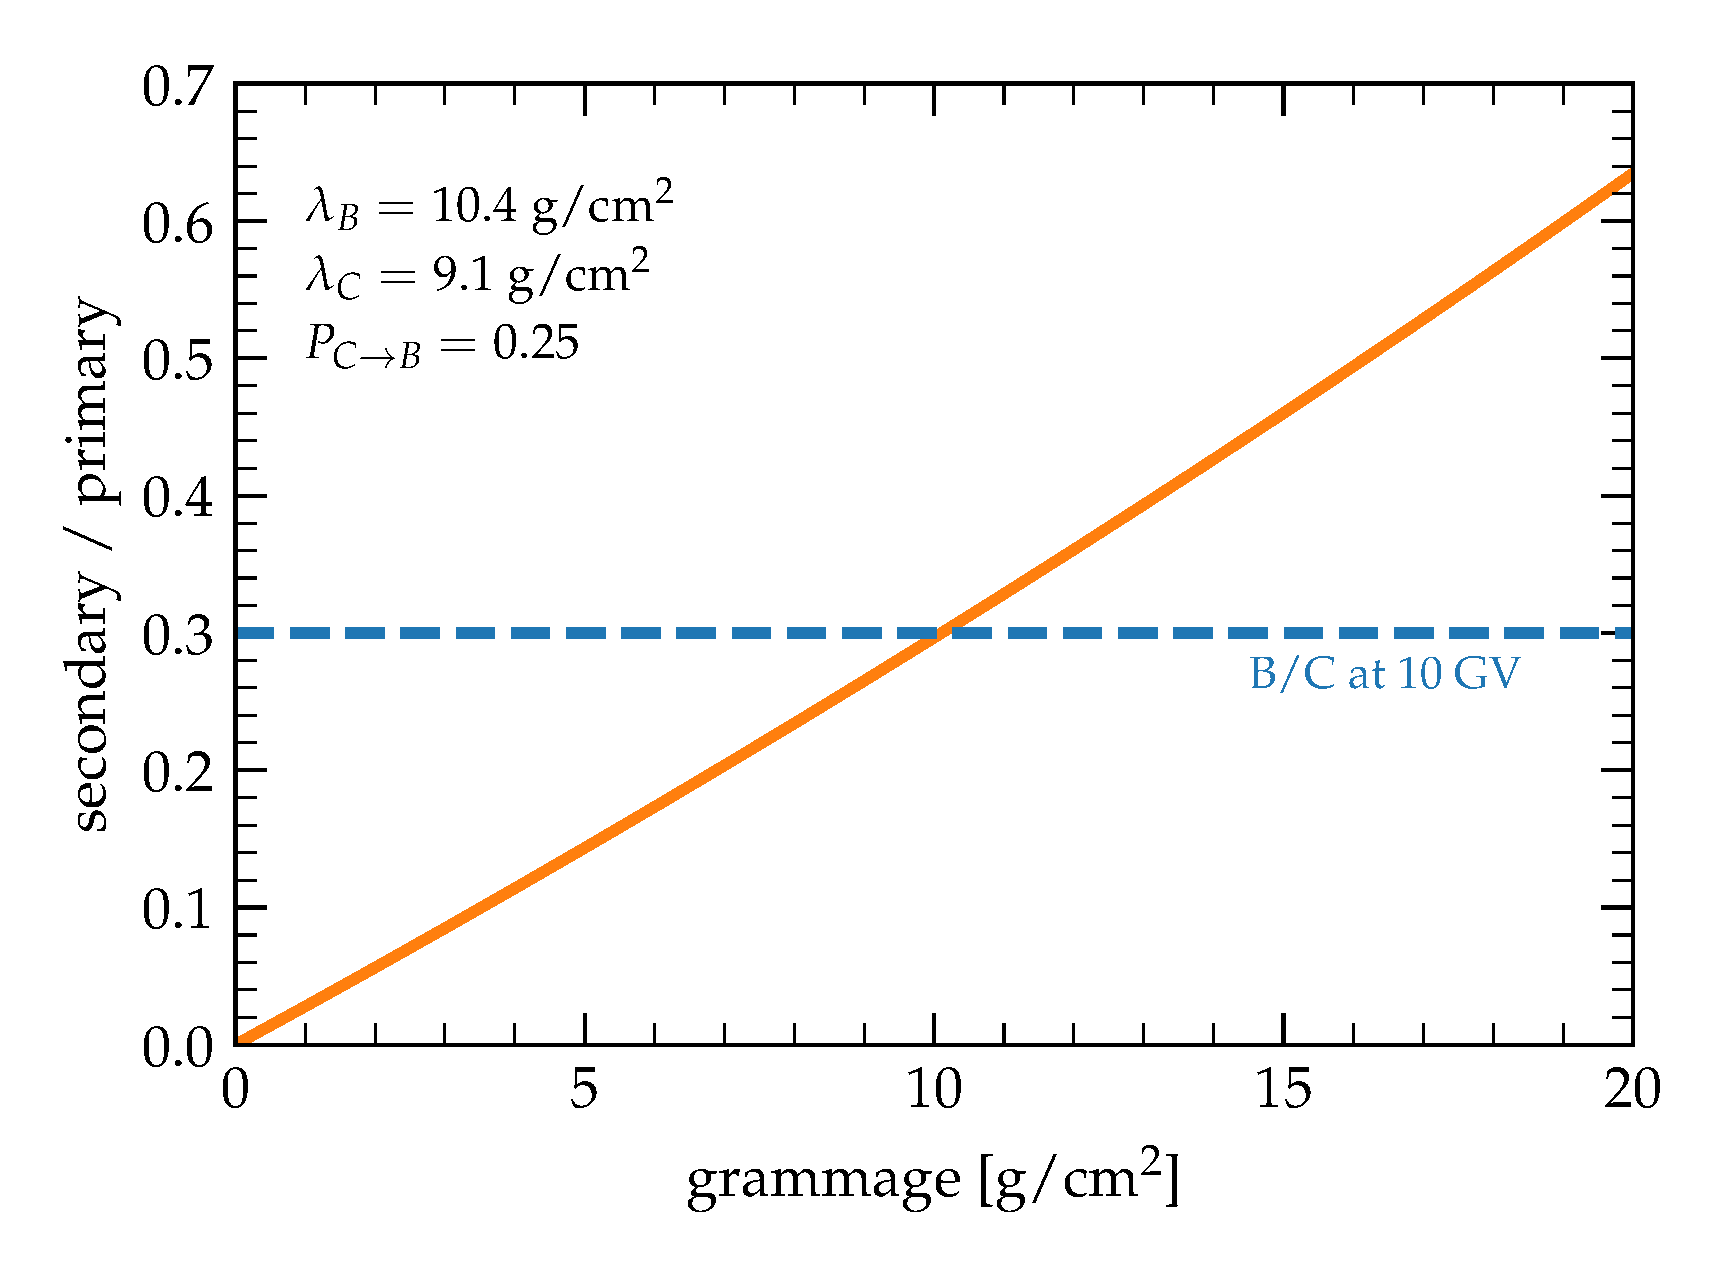
\includegraphics[width=0.6\textwidth]{figures/grammage_simple.pdf} 
\caption{The ratio of secondary to primary cosmic rays (B/C) as a function of grammage as in~\cref{eq:grammagesimple}. The dotted blue line show the measurement by AMS-02 for CRs with rigidities \(R \sim 10~\text{GV}\).}
\label{fig:grammage10}
\end{figure}

\subsection{Galactic Disk Grammage and Confinement Time}

To estimate the grammage accumulated by CRs as they propagate, let us first compute the grammage associated with a single crossing of the Galactic gas disk, \(\chi_d\). This grammage is approximately the average surface density of the Galactic disk: \(\mu_d \sim 2.3 \times 10^{-3}~\text{g/cm}^2\).  

However, this value is significantly smaller than the \(\sim 10~\text{g/cm}^2\) inferred from the B/C ratio. This stark discrepancy indicates that CRs must traverse the disk \emph{multiple times} to accumulate the observed grammage.  

As such, to quantify the confinement time, we calculate the total time CRs need to cross the disk to accumulate the required grammage. This timescale is given by the number of crossings multiplied by the time for a single crossing:  
\[
\tau_{\rm conf} \gtrsim \frac{\chi_{\rm ISM}}{\chi_d} \frac{2h}{v} \sim 3 \times 10^6~\text{yr},
\]
where \(h \sim 100~\text{pc}\) is the half-thickness of the Galactic disk, and \(v \sim c\) is the approximate velocity of CRs.  

This \emph{minimum confinement timescale}, \(\tau_{\rm conf} \sim 3 \times 10^6~\text{yr}\), is several orders of magnitude longer than the time required for a CR to traverse the Galaxy in a straight line at the speed of light (a few tens of kiloyears for \(\sim 10~\text{kpc}\)). This vast difference provides compelling evidence for \emph{efficient confinement mechanisms} that cause CRs to propagate diffusively rather than ballistically through the Galaxy.  

The total residence time of CRs in the Galaxy can be independently estimated using radioactive isotopes such as \(^{10}\text{Be}\), which has a decay lifetime comparable to the timescale for CR leakage from the Galaxy. The ratio of radioactive \(^{10}\text{Be}\) to stable \(^{9}\text{Be}\) measured in CRs suggests a mean residence time of:  
\[
\tau_H \sim 10^8~\text{yr}.
\]  

Combining this estimate with the B/C ratio provides additional insights into CR propagation. To avoid exceeding the observed grammage, CRs must spend most of their time in the \emph{low-density Galactic halo}, where the density is much lower than in the disk. This requirement can be expressed as:  
\[
\langle \rho \rangle \lesssim \frac{\mu_d}{2h} \frac{\tau_h}{\tau_H}.
\]  
Here, \(\tau_h\) is the confinement time in the disk, and \(\tau_H\) is the total residence time in the Galaxy. This inequality implies that CRs interact predominantly with the disk during their brief crossings but spend the majority of their residence time in the halo.  

In conclusion, the composition of CRs, particularly the observed ratios of secondaries to primaries (e.g., B/C), provides robust evidence for efficient confinement mechanisms that ensure CRs propagate diffusively through the Galaxy. This confinement allows CRs to \emph{repeatedly return to the disk}, producing the observed secondary components, while spending most of their time in the low-density Galactic halo.

In the remainder of this chapter, we will explore transport models that explain these observations in terms of phenomenological quantities such as the diffusion coefficient and the size of the halo.  
